\documentclass[10pt]{article}
\newcommand{\doctitle}{System Architecture \& Design Document}
% Shared layout for the CTRL ALT DEFEAT documents (compile with xelatex).
\usepackage{fontspec}
\setmainfont{TeX Gyre Termes}
\setsansfont{TeX Gyre Heros}
\setmonofont{DejaVu Sans Mono}[Scale=0.80]
\usepackage[letterpaper, top=0.72in, bottom=0.78in, left=0.8in, right=0.8in,
            headheight=13pt, headsep=9pt, footskip=22pt]{geometry}
\usepackage{microtype}
\linespread{1.02}
\usepackage{xcolor}
\definecolor{ink}{HTML}{1F2A44}
\definecolor{accent}{HTML}{3B5B92}
\definecolor{attc}{HTML}{3B5B92}
\definecolor{attf}{HTML}{E8EFF9}
\definecolor{txtc}{HTML}{B5651D}
\definecolor{txtf}{HTML}{FDF0E2}
\definecolor{evalc}{HTML}{3C7A50}
\definecolor{evalf}{HTML}{E6F3EA}
\definecolor{rulec}{HTML}{C9D3E3}
\definecolor{shade}{HTML}{F4F7FB}
\usepackage{titlesec}
\titleformat{\section}{\sffamily\bfseries\large\color{ink}}{\thesection}{0.55em}{}
\titlespacing*{\section}{0pt}{8pt}{2pt}
\titleformat{\subsection}[runin]{\sffamily\bfseries\normalsize\color{ink}}{\thesubsection}{0.45em}{}[.]
\titlespacing*{\subsection}{0pt}{4pt}{0.55em}
\usepackage{enumitem}
\setlist{nosep, leftmargin=1.15em, topsep=1pt, itemsep=1pt}
\usepackage{booktabs, tabularx, array, multirow, makecell}
\renewcommand{\arraystretch}{1.12}
\newcolumntype{L}{>{\raggedright\arraybackslash}X}
\newcolumntype{P}[1]{>{\raggedright\arraybackslash}p{#1}}
\usepackage{graphicx}
\usepackage{caption}
\captionsetup{font={small,sf}, labelfont={bf,color=ink}, skip=3pt}
\usepackage{float}
\usepackage{tikz}
\usetikzlibrary{arrows.meta, positioning, calc, fit, backgrounds}
\usepackage{listings}
\lstset{basicstyle=\ttfamily\scriptsize, columns=fullflexible, keepspaces=true, breaklines=true,
        frame=single, rulecolor=\color{rulec}, backgroundcolor=\color{shade}, framesep=3pt,
        xleftmargin=3pt, xrightmargin=3pt, aboveskip=3pt, belowskip=3pt, showstringspaces=false,
        breakatwhitespace=true, upquote=true}
\usepackage{fancyhdr, lastpage}
\pagestyle{fancy}
\fancyhf{}
\renewcommand{\headrulewidth}{0.4pt}
\fancyhead[L]{\sffamily\footnotesize\color{ink}CTRL ALT DEFEAT \textbullet\ \doctitle}
\fancyhead[R]{\sffamily\footnotesize\color{ink}CS 6338 Knowledge Engineering}
\fancyfoot[C]{\sffamily\footnotesize\color{ink}Page \thepage\ of \pageref{LastPage}}
\fancypagestyle{first}{\fancyhf{}\renewcommand{\headrulewidth}{0pt}%
  \fancyfoot[C]{\sffamily\footnotesize\color{ink}Page \thepage\ of \pageref{LastPage}}}
\usepackage[hidelinks]{hyperref}
\setlength{\parindent}{0pt}
\setlength{\parskip}{3pt}
\newcommand{\code}[1]{\texttt{#1}}
\renewcommand{\cite}[1]{[#1]}
% A small rounded label for the subsystem numbers in the figures
\newcommand{\badge}[1]{\tikz[baseline=(b.base)]\node[circle, fill=ink, text=white, inner sep=1pt,
  minimum size=9pt, font=\sffamily\bfseries\tiny](b){#1};}
\tikzset{
  box/.style={draw, rounded corners=2.5pt, align=center, inner sep=3pt, font=\sffamily\scriptsize, line width=0.6pt,
    execute at begin node={\hyphenpenalty=10000\exhyphenpenalty=10000\relax}},
  txtbox/.style={box, draw=txtc, fill=txtf},
  attbox/.style={box, draw=attc, fill=attf},
  evalbox/.style={box, draw=evalc, fill=evalf},
  plainbox/.style={box, draw=ink!60, fill=white},
  flow/.style={-{Stealth[length=4pt, width=3.4pt]}, line width=0.6pt, draw=ink!75},
  rel/.style={-{Stealth[length=4pt, width=3.4pt]}, line width=0.6pt},
  lab/.style={font=\sffamily\tiny, fill=white, inner sep=0.8pt},
}

\usepackage{amsmath, amssymb, xltabular}
\hypersetup{pdftitle={CTRL ALT DEFEAT: GraphRAG System Architecture and Design Document}, pdfauthor={Shane Waldrop}}
\lstdefinelanguage{cypher}{morekeywords={CYPHER,MATCH,WHERE,WITH,RETURN,CALL,YIELD,UNWIND,MERGE,SET,CREATE,CONSTRAINT,INDEX,VECTOR,FOR,ON,REQUIRE,IS,UNIQUE,IF,NOT,EXISTS,OPTIONS,AS,AND,IN,ORDER,BY,DESC,LIMIT,SEARCH,SCORE,DISTINCT},sensitive=true,morestring=[b]',morecomment=[l]{//}}
\lstset{basicstyle=\ttfamily\fontsize{8.75}{10}\selectfont, keywordstyle=\bfseries, postbreak=\mbox{\textcolor{accent}{$\hookrightarrow$}\ }, moredelim=[is][\sffamily\itshape\color{accent}]{@@}{@@}}
% a class box: bold name, a rule, then the members
\newcommand{\cls}[2]{\textbf{#1}\\[-2pt]\rule{\linewidth}{0.3pt}\\#2}
\renewcommand{\badge}[1]{\tikz[baseline=(b.base)]\node[circle, fill=ink, text=white, inner sep=0.6pt, minimum size=10.5pt, font=\sffamily\bfseries\scriptsize](b){#1};}
\newcommand{\figcode}{\renewcommand{\code}[1]{\textsf{##1}}}

\begin{document}
\thispagestyle{first}
{\sffamily
{\color{accent}\footnotesize\bfseries CS 6338 KNOWLEDGE ENGINEERING \textbullet\ TERM PROJECT DESIGN DOCUMENT (MILESTONE 2)}\par\vspace{2pt}
{\color{ink}\LARGE\bfseries GraphRAG over Cyber Threat Reports: System Architecture \& Design}\par\vspace{3pt}
{\small Team \textbf{CTRL ALT DEFEAT} \textbullet\ Shane Waldrop (swaldrop2@angelo.edu)\\ Angelo State University \textbullet\ Instructor: Dr.\ Erdogan Dogdu \textbullet\ October 2026}\par}
\vspace{4pt}
\noindent\colorbox{shade}{\parbox{\dimexpr\textwidth-2\fboxsep}{\small
\textbf{Scope.} This document specifies every module of a GraphRAG (graph retrieval-augmented generation) system. An analyst asks a multi-hop question about cyber threat reports, meaning a question whose answer joins several linked facts. The system answers from retrieved report text and from a Neo4j knowledge graph that joins the AnnoCTR threat reports \cite{1} with MITRE ATT\&CK (Adversarial Tactics, Techniques, and Common Knowledge) version 20.0 \cite{11}. The model is told to cite the report chunk or graph relationship behind each statement, and code checks that every cited ID was in the model's context. Every result is labelled \emph{measured} (with its date), \emph{estimated}, \emph{planned} or \emph{target}; counts describe the data and code at the cited commit.
\textbf{Built and run on the target laptop by 19 October 2026:} the schema, ATT\&CK loading, extraction, entity linking, loading and question answering for one development (dev) report, the \emph{tracer report} (Lab52's June 2020 report on Mustang Panda, run end to end as the first test); the benchmark; the scorer. \textbf{Planned for the full build} (Phase 5, all 16 dev and 34 test reports): the report lookup and summary lines of Section~6, GDS (Neo4j Graph Data Science) analytics, the node vector indexes and the chat page (the application programming interface (API) routes of Section~8 are a specification only); then, in the evaluation (Phase 6), RAGAS (Retrieval-Augmented Generation Assessment) scoring and the human ratings.}}

\vspace{2pt}
\begin{table}[H]\centering\small
\caption{Repository checkpoint: \url{https://github.com/Wittyusername12/ctrl-alt-defeat-graphrag} (public; branch \code{build}, commit \code{2d7a06f} of 19 October 2026).}\label{tab:checkpoint}
\begin{tabularx}{\textwidth}{@{}P{5.3cm}L@{}}
\toprule
Required item & Files\\
\midrule
Database initialization and schema & \code{schema.cypher} (8 uniqueness constraints, chunk vector index); \code{schemas.py} (labels, relationship types, keys and shared property names, each defined once); \code{apply\_schema.py}; \code{load\_attack.py}\\
LLM (large language model) extraction prompts and parser tests & \code{extract.py} (prompt, two worked examples, reply checks); \code{tests/test\_pipeline\_logic.py} (valid reply, bad JSON (JavaScript Object Notation), evidence not in the chunk, wrong direction, every drop reason)\\
Ground-truth benchmark files & \code{benchmark/gold\_triples.json} (682 triples); \code{benchmark/eval\_queries.json} (24 multi-hop question--answer pairs); both written by \code{gold.py} and checked by \code{tests/test\_gold.py}\\
Data models and scoring & \code{models.py}, \code{extract.py} (Pydantic models: Python classes that validate data); \code{score.py} with \code{tests/test\_score.py}; 86 tests in all\\
\bottomrule
\end{tabularx}
\end{table}

\section{Executive Summary \& System Requirements}
\textbf{Domain and persona.} Cyber threat intelligence (CTI). The user is a security operations center (SOC) or CTI analyst who reads vendor threat reports, maps them to ATT\&CK, and decides which detections and mitigations to prioritise. The analyst needs answers that combine what a report says with what ATT\&CK records, and needs every claim traceable to its source.

\begingroup\small
\begin{xltabular}{\textwidth}{@{}p{0.85cm}L@{}}
\caption{Functional (FR) and non-functional (NFR) requirements.}\label{tab:req}\\
\toprule
\endfirsthead
\toprule
\endhead
\bottomrule
\endlastfoot
FR1 & Ingest AnnoCTR reports: remove embedded images; split each report into 4,000-character chunks with 400 characters of overlap.\\
FR2 & Extract technique, tactic, group and software mentions and ``uses'' relations from each chunk with an LLM, each with its verbatim evidence sentence, in a reply whose format a JSON schema enforces.\\
FR3 & Resolve every mention to an ATT\&CK v20.0 entry (named entity disambiguation, NED) or to an Entity node, recording the method and the confidence.\\
FR4 & Load ATT\&CK v20.0 from its STIX (Structured Threat Information Expression) file through RDF/OWL (Resource Description Framework / Web Ontology Language, built with rdflib) into Neo4j, checking every count.\\
FR5 & Answer multi-hop questions: look up the report a question names, search chunk vectors, then take a personalized-PageRank subgraph around the entities found, with link counts computed in Cypher (Neo4j's query language); all of it runs as Cypher and GDS calls when the question arrives.\\
FR6 & Tell the model to cite \code{[chunk:ID]} or \code{[edge:ID]} after every statement; check that each cited ID was in the context, and flag a GraphRAG answer that cites nothing; answer the same question without the graph (the baseline).\\
FR7 & Run GDS PageRank, Louvain and FastRP (fast random projection); index chunk and node embeddings (lists of numbers that place similar items close together).\\
FR8 & Evaluate entity extraction and linking against gold labels, answer accuracy, RAGAS metrics and blind human ratings; show answers, citations and context in a chat page.\\
\midrule
NFR1 & Latency (target): median under 10\,s per question, end to end. Measured 19 Oct: the one GraphRAG answer call took 3.72\,s (the baseline's 1.96\,s). The other stages are not yet timed, so GraphRAG will exceed the assignment's 3\,s example end to end (inference).\\
NFR2 & Cost: every model reply is saved under the SHA-256 cryptographic hash of its request and reused, so a rerun costs nothing. Measured token counts at list prices (\$2 and \$10 per million input and output tokens for gpt-6-sol) put the tracer report, end to end, at about \$0.07. Estimated: about \$3.8 to extract all 149 dev and test chunks (the tracer's 2 chunks used 5,081 tokens in and 3,430 out, \$0.044; the second worked example adds about 1,550 input tokens a request, at the tracer's 3.7 characters per token); roughly \$30--45 for the RAGAS judge, the largest expense (288 calls to gpt-6-astra at \$10 and \$50 per million tokens, its reasoning billed as output), to be measured first on a 2-question trial.\\
NFR3 & Throughput: measured 8--14\,s per chunk with gpt-6-sol, so the 149 dev and test chunks take an estimated 20--35 minutes one after another ($149 \times 8$ to $14$\,s).\\
NFR4 & Reproducibility: 120 pinned packages; saved replies; temperature 0 and seed 7; GDS runs with one thread (personalized PageRank today, the analytics when built) and FastRP with a fixed seed; analytics results saved to files (planned). Measured: the benchmark rebuilds byte-identically on Windows and Linux.\\
NFR5 & Security: the OpenAI key and the Neo4j password live only in a git-ignored \code{.env} file, read by explicit path; Neo4j listens on localhost only.\\
\end{xltabular}
\endgroup

\section{End-to-End System Architecture}
\begin{figure}[H]\centering\figcode
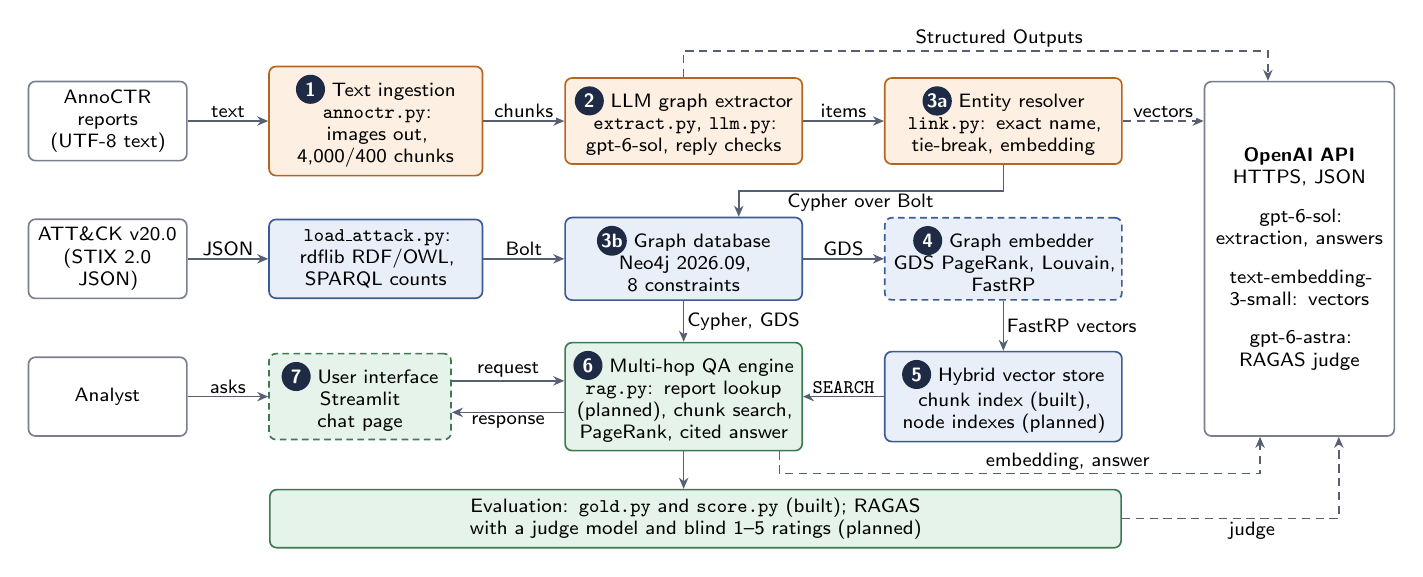
\begin{tikzpicture}[x=1cm, y=1cm]
\tikzset{c1/.style={text width=1.8cm, minimum height=1.0cm}, c2/.style={text width=2.5cm, minimum height=1.0cm},
  c3/.style={text width=2.8cm, minimum height=1.0cm}, planned/.style={dash pattern=on 2.4pt off 1.6pt},
  elab/.style={font=\sffamily\scriptsize, fill=white, inner sep=1pt}, call/.style={flow, dash pattern=on 3pt off 2pt}}
\node[plainbox, c1] (src) at (1.01,0) {AnnoCTR reports\\(UTF-8 text)};
\node[txtbox, c2] (ing) at (4.415,0) {\badge{1} Text ingestion\\\code{annoctr.py}: images out,\\4,000/400 chunks};
\node[txtbox, c3] (ext) at (8.325,0) {\badge{2} LLM graph extractor\\\code{extract.py}, \code{llm.py}:\\gpt-6-sol, reply checks};
\node[txtbox, c3] (ned) at (12.385,0) {\badge{3a} Entity resolver\\\code{link.py}: exact name,\\tie-break, embedding};
\node[plainbox, text width=2.2cm, minimum height=4.5cm] (oai) at (16.145,-1.75) {\textbf{OpenAI API}\\HTTPS, JSON\\[6pt]gpt-6-sol:\\extraction, answers\\[6pt]text-embedding-\\3-small: vectors\\[6pt]gpt-6-astra:\\RAGAS judge};
\node[plainbox, c1] (stix) at (1.01,-1.75) {ATT\&CK v20.0\\(STIX 2.0 JSON)};
\node[attbox, c2] (rdf) at (4.415,-1.75) {\code{load\_attack.py}:\\rdflib RDF/OWL,\\SPARQL counts};
\node[attbox, c3] (neo) at (8.325,-1.75) {\badge{3b} Graph database\\Neo4j 2026.09,\\8 constraints};
\node[attbox, c3, planned] (emb) at (12.385,-1.75) {\badge{4} Graph embedder\\GDS PageRank, Louvain,\\FastRP};
\node[plainbox, c1] (an) at (1.01,-3.5) {Analyst};
\node[evalbox, text width=2.1cm, minimum height=1.0cm, planned] (ui) at (4.215,-3.5) {\badge{7} User interface\\Streamlit chat page};
\node[evalbox, c3] (qa) at (8.325,-3.5) {\badge{6} Multi-hop QA engine\\\code{rag.py}: report lookup\\(planned), chunk search,\\PageRank, cited answer};
\node[attbox, c3] (vec) at (12.385,-3.5) {\badge{5} Hybrid vector store\\chunk index (built),\\node indexes (planned)};
\node[evalbox, text width=10.6cm, minimum height=0.6cm] (ev) at (8.475,-5.05) {Evaluation: \code{gold.py} and \code{score.py} (built); RAGAS with a judge model and blind 1--5 ratings (planned)};
\draw[flow] (src) -- node[elab, above]{text} (ing);
\draw[flow] (ing) -- node[elab, above]{chunks} (ext);
\draw[flow] (ext) -- node[elab, above]{items} (ned);
\draw[flow] (stix) -- node[elab, above]{JSON} (rdf);
\draw[flow] (rdf) -- node[elab, above]{Bolt} (neo);
\draw[flow] (neo) -- node[elab, above]{GDS} (emb);
\draw[flow] (ned.south) -- ++(0,-0.33) -| node[elab, pos=0.27, below]{Cypher over Bolt} ($(neo.north)+(0.7,0)$);
\draw[flow] (emb.south) -- node[elab, right]{FastRP vectors} (vec.north);
\draw[flow] (vec) -- node[elab, above]{\code{SEARCH}} (qa);
\draw[flow] (neo.south) -- node[elab, right]{Cypher, GDS} (qa.north);
\draw[flow] (an) -- node[elab, above]{asks} (ui);
\draw[flow] ($(ui.east)+(0,0.2)$) -- node[elab, above]{request} ($(qa.west)+(0,0.2)$);
\draw[flow] ($(qa.west)+(0,-0.2)$) -- node[elab, below]{response} ($(ui.east)+(0,-0.2)$);
\draw[flow] (qa.south) -- (qa.south |- ev.north);
\draw[call] (ext.north) -- ++(0,0.33) -| node[elab, pos=0.27, above]{Structured Outputs} ($(oai.north)+(-0.4,0)$);
\draw[call] (ned) -- node[elab, above]{vectors} (ned -| oai.west);
\draw[call] ($(qa.south east)+(-0.3,0)$) -- ++(0,-0.28) -| node[elab, pos=0.3, above]{embedding, answer} ($(oai.south)+(-0.5,0)$);
\draw[call] (ev.east) -| node[elab, pos=0.3, below]{judge} ($(oai.south)+(0.5,0)$);
\end{tikzpicture}
\caption{Component diagram. Numbered boxes are the seven subsystems the assignment names: 1 text ingestion, 2 LLM graph extractor, 3a entity resolver and 3b graph database, 4 graph embedder, 5 hybrid vector store, 6 multi-hop question-answering (QA) engine, 7 user interface. Dashed outline: not built yet. Dashed arrow: an HTTPS (Hypertext Transfer Protocol Secure) call to the OpenAI application programming interface (API). Neo4j holds the graph and every vector index, so 3b and 5 are one database. Bolt is Neo4j's binary network protocol; SPARQL (SPARQL Protocol and RDF Query Language) queries RDF graphs.}\label{fig:arch}
\end{figure}

\begin{table}[tb]\centering\small
\caption{Data flow between modules (Bolt is Neo4j's binary network protocol).}\label{tab:flows}
\begin{tabularx}{\textwidth}{@{}P{2.45cm}LLP{2.75cm}@{}}
\toprule
Connection & Input & Output & Protocol, format\\
\midrule
1 $\rightarrow$ 2 & report text (UTF-8 Unicode, embedded images removed) & chunks: \code{chunk\_id} = \code{<report\_id>\#<index>}, start, end, text & in-process Python calls\\
2 $\leftrightarrow$ OpenAI & system prompt, two worked examples, chunk; JSON schema from Pydantic & JSON reply, saved as \code{replies/extract/<SHA-256>.json} & HTTPS, Chat Completions with Structured Outputs\\
2 $\rightarrow$ 3a & kept mentions and relations; counts of 13 drop reasons & per mention: ATT\&CK ID or Entity, method, confidence & in-process Python calls\\
3a $\leftrightarrow$ OpenAI & mention texts, chunk texts, ATT\&CK entry texts & 1,536-number embeddings, saved as \code{.npz} files & HTTPS, Embeddings\\
3a $\rightarrow$ 3b & report; chunks with embeddings; MENTIONS; text USES & nodes and relationships, read back and counted & Cypher 25 over Bolt, 1,000 rows a batch\\
STIX $\rightarrow$ 3b & 1,785 live objects; 19,545 relationship objects plus 881 technique-to-tactic links from kill-chain phases & 194,611 RDF triples (Turtle file); 1,785 nodes and 20,426 relationships, read back & rdflib, then Bolt\\
3b $\rightarrow$ 4 $\rightarrow$ 5 & projected ATT\&CK graph (planned) & PageRank score, community, 128-number FastRP vector per node; saved to files; a vector index for each of Technique, Group and Software & GDS procedures, Cypher\\
6 $\leftrightarrow$ 3b, 5, OpenAI & question and its embedding & anchored reports (planned), chunks, seeds, PageRank scores, summary lines (planned), fact lines; answer text with citations & \code{SEARCH} subclause, GDS, HTTPS\\
7 $\leftrightarrow$ 6 & \code{QueryRequest} (planned) & \code{QueryResponse} (Section~\ref{sec:models}) & in-process calls; HTTP route specification (Table~\ref{tab:api})\\
Evaluation $\leftrightarrow$ OpenAI & question, answer, contexts, reference answer (planned) & RAGAS scores; judge replies cached & HTTPS\\
\bottomrule
\end{tabularx}
\end{table}

\section{Graph Extraction \& Schema Engineering Pipeline}
\textbf{Domain schema.} Node types and keys (each key has a uniqueness constraint): Report (\code{report\_id}; vendor, date, title, split, characters); Chunk (\code{chunk\_id}; report\_id, index, start, end, text, embedding); the five ATT\&CK classes Technique, Tactic, Group, Software and Mitigation (\code{attack\_id}; name, description, url, stix\_id; aliases on groups and software; Technique \code{is\_subtechnique}, Software \code{software\_type}, Tactic \code{shortname}); and Entity (\code{entity\_id} = category:normalised name; name, category), for a name that links to no ATT\&CK entry. Table~\ref{tab:rels} lists the relationship predicates; every relationship carries \code{edge\_id} (the ID an answer cites) and \code{source} (\code{attack} or \code{text}).

\begin{table}[tb]\centering\small
\caption{Relationship predicates (ATT\&CK counts measured after loading, 18 Oct).}\label{tab:rels}
\begin{tabularx}{\textwidth}{@{}P{3.1cm}P{4.7cm}L@{}}
\toprule
Predicate & From $\rightarrow$ to & Properties besides \code{edge\_id} and \code{source}\\
\midrule
HAS\_CHUNK & Report $\rightarrow$ Chunk & none\\
MENTIONS & Chunk $\rightarrow$ any ATT\&CK node, or Entity & report\_id, chunk\_id, mention\_text, evidence, category, attack\_name, link\_method, confidence, model\_confidence, model, reply\_key, extracted\\
USES & ATT\&CK: Group $\rightarrow$ Technique (4,815), Software $\rightarrow$ Technique (11,608), Group $\rightarrow$ Software (1,166); text: from the node a group or software mention links to, to the node a technique or software mention links to (any ATT\&CK label, or Entity) & ATT\&CK: stix\_id, description. Text: report\_id, chunk\_id, evidence, reply\_key\\
SUBTECHNIQUE\_OF & Technique $\rightarrow$ Technique (479) & stix\_id\\
PART\_OF\_TACTIC & Technique $\rightarrow$ Tactic (881) & none (read from each technique's kill-chain phases)\\
MITIGATES & Mitigation $\rightarrow$ Technique (1,477) & stix\_id, description\\
\bottomrule
\end{tabularx}
\end{table}

\textbf{Chunking.} Chunk $i$ spans characters $[3600\,i,\ \min(3600\,i + 4000, L))$ of a report with $L$ characters, for $i = 0$ and every further $i$ with $3600\,i < L - 400$. Neighbouring chunks share 400 characters, so a sentence of up to 400 characters that crosses a boundary is whole in one of the two chunks. Counts: train 228, dev 50, test 99 chunks.

\textbf{Prompt specification.} Each request holds six messages: (1) the system prompt below; (2)--(5) two worked examples, each a user message ``Chunk:'' followed by the opening of a train report and an assistant message holding the reply to it, written by hand and checked to pass every rule below; (6) a user message ``Chunk:'' followed by the chunk. The first example is the first 1,064 characters of \code{intel471\_2020-12-18\_}\allowbreak\code{ta505-get2-loader-malware-december} (12 mentions, 2 relations: techniques described rather than named, and a tactic). The second is the first 1,293 characters of \code{zscaler\_2020-09-29\_}\allowbreak\code{spear-phishing-campaign-delivers-buer} (16 mentions, 2 relations: a sub-technique, software with no ATT\&CK entry, a group named after its malware, and two names joined by ``worked with'', which is no ``uses'' relation). OpenAI Structured Outputs enforces the reply format with the JSON schema of \code{ChunkExtraction} (Section~\ref{sec:models}); the reply models carry no value constraints (Structured Outputs accepts no string-length limits), and code checks the ids, texts, evidence sentences and relations instead. Settings: gpt-6-sol, reasoning effort none, temperature 0, seed 7, at most 4,000 completion tokens. The system prompt, exactly (\textcolor{accent}{$\hookrightarrow$} marks a line wrapped to fit the page):
\begin{lstlisting}
You read one chunk of a cyber threat report and list the MITRE ATT&CK Enterprise concepts in it.

Concepts:
- technique: an adversary behaviour, whether the chunk names the ATT&CK technique or only describes the behaviour
- tactic: an adversary goal, such as Execution, Persistence or Command and Control
- group: a named threat actor
- software: a named piece of malware or a named tool

List one entry for each place where the chunk names or describes a concept:
- id: m1, m2, m3 and so on, in the order the entries appear in the chunk
- text: the words in the chunk that name or describe the concept, copied exactly
- category: technique, tactic, group or software
- attack_name: the concept's name in ATT&CK Enterprise version 20, spelled as ATT&CK spells it; for a sub-technique write "Parent technique: Sub-technique"; write "" when no ATT&CK entry fits
- evidence: the whole sentence of the chunk that contains the text, copied exactly
- confidence: a number from 0 to 1 saying how sure you are of attack_name

Then list each "uses" relation: a group or a piece of software (user) uses a technique or a piece of software (used). List a relation only when its evidence sentence names or clearly refers to both, and refer to both by their entry ids.

Copy text and evidence character for character from the chunk. Every entry must rest on the chunk's own words; use your knowledge of ATT&CK only to choose attack_name. Some version 20 names differ from older versions: for example, the tactic once called Defense Evasion is now Stealth (hiding activity) or Defense Impairment (breaking defences). Organisations, people, places, file names, and indicators such as addresses or hashes are not concepts.
\end{lstlisting}
The 19 October tracer run used one worked example and an earlier wording of the version-20 sentence (``Some names changed in version 20''), corrected because those names already existed before version 20. Every tracer figure in this document comes from that run, whose saved replies match commit \code{7cacf7b}; the full build reruns the report with the prompt above.

\textbf{Confidence thresholds and malformed output.} The model writes local ids (m1, m2, \ldots) only; code assigns every permanent ID (\code{<report\_id>\#<index>/m3}). Each reply is saved before it is checked, including cut-off, filtered and malformed replies. An item is dropped, and the reason counted, when: the content filter stopped the reply; the model refused; the reply hit the token cap; the reply is not valid JSON in the schema; a mention id repeats; a mention text is empty; the text is not in the chunk; the evidence is not in the chunk; the text is not in its evidence; a relation names a missing or dropped mention; a relation points the wrong way (technique uses group); the two categories cannot use each other; or the relation's evidence is not in the chunk. Text comparisons treat typographic quotes, dashes and runs of white space as their plain forms. Measured on the tracer report (19 Oct): 29 mentions and 9 relations kept, 0 dropped. Link confidence is 1.0 for an exact name match and the cosine similarity for an embedding match. An embedding match is accepted at cosine $\ge \tau$. The provisional $\tau = 0.40$ accepts every embedding match seen so far (the tracer's six had cosines 0.696--0.783), so the full build sets $\tau$ on the 213 dev facts (planned: the value that gives the highest dev F1 score, the harmonic mean of precision and recall). The model's own confidence is stored and not yet used. On the tracer report it ranged from 0.3 to 1.0, and at parent level 7 of the 8 links outside the gold had 0.9 or less, against 2 of the 21 gold links; one report is no calibration, so the dev calibration also tests a cut-off on that confidence (planned).

\textbf{Entity resolution and deduplication.} \code{link.py} resolves each kept mention in four steps.
(1) Normalise names: plain quotes and dashes, single spaces, lower case, outer punctuation removed.
(2) Look up the model's \code{attack\_name}, then the mention text, among 2,927 keys: the 2,448 distinct normalised ATT\&CK names and aliases plus the 479 ``Parent: Sub-technique'' names, across all five ATT\&CK kinds, never only the kind the model guessed.
(3) When a key names several entries (49 keys; for example ``Carbanak'' names a group and a piece of software), the model's category breaks the tie, then the parent named in ``Parent: Sub-technique''; otherwise the mention goes to step 4. No tie is settled by an arbitrary pick.
(4) Embed the mention's \code{attack\_name}, text and evidence sentence, joined by full stops, with text-embedding-3-small and compare the vector with every entry's ``name: description'' (citation markers removed, links reduced to their text, at most 4,000 characters). Link the closest entry at cosine $\ge \tau$; otherwise create an Entity node keyed \code{category:normalised name}, so repeated unlinked names merge into one node. Measured on the tracer report (19 Oct): 23 exact and 6 embedding links. In all 6 the model had written ``Hijack Execution Flow: DLL Side-Loading'', the name of T1574.002, which ATT\&CK revoked in favour of T1574.001 ``DLL'' (dynamic-link library); the embedding step linked all 6 to T1574.001, at cosine 0.696--0.783.

\section{Graph Storage, Enhancement \& Reasoning Engine}
\textbf{Database setup.} Neo4j 2026.09 Enterprise runs in Neo4j Desktop 2.2.1 with APOC (Awesome Procedures On Cypher) and GDS 2026.09. The script \code{apply\_schema.py} applies \code{schema.cypher} (8 constraints, then the vector index, waiting until it is ONLINE) before any load, and \code{load\_attack.py} checks that the constraints exist before it writes. Neo4j backs each uniqueness constraint with a range index, so every lookup by key (each \code{MERGE} in the loaders, each report and chunk lookup) uses an index. Every data query starts with \code{CYPHER 25}; writes use \code{MERGE} (Cypher's create-if-absent) in batches of 1,000, so a rerun changes nothing; reloading a report first removes that report's text-derived nodes and relationships.
\begin{lstlisting}[language=cypher]
CREATE CONSTRAINT technique_key IF NOT EXISTS FOR (n:Technique) REQUIRE n.attack_id IS UNIQUE;   // one per label: 8 in all
CREATE VECTOR INDEX chunk_embedding IF NOT EXISTS FOR (n:Chunk) ON (n.embedding)
OPTIONS {indexConfig: {`vector.dimensions`: 1536, `vector.similarity_function`: 'cosine', `vector.quantization.type`: 'NONE'}};
\end{lstlisting}

\textbf{Reasoning layer 1: data fusion with ATT\&CK.} \code{load\_attack.py} integrates the external ATT\&CK database: (1) it checks the STIX file's SHA-256 hash; (2) it keeps live objects (neither revoked nor deprecated) of five kinds and their \code{uses}, \code{mitigates} and \code{subtechnique-of} relationships, plus technique-to-tactic links from kill-chain phases; (3) it builds an RDF/OWL graph with rdflib (OWL classes and object properties; each relationship is also an \code{rdf:Statement} carrying its ID and description, because RDF 1.1 cannot attach properties to a triple) and saves the graph as Turtle, a text format for RDF; (4) it counts the classes with SPARQL and compares every count with the STIX file; (5) it writes the nodes and relationships, taken from the RDF graph, to Neo4j and reads the counts back. Measured (18 Oct): 194,611 triples; 1,785 nodes and 20,426 relationships, equal at every stage. Report facts join this graph through the entity resolver, so one Cypher path runs from a report sentence to an ATT\&CK mitigation.

\textbf{Reasoning layer 2: hierarchy inference rule.} A relationship that ATT\&CK records for a sub-technique also holds for its parent technique:
$\mathit{USES}(x, s) \wedge \mathit{SUBTECHNIQUE\_OF}(s, t) \Rightarrow \mathit{USES}(x, t)$, and likewise for MITIGATES. The rule matters here: 8,877 of ATT\&CK's 16,423 USES relationships to techniques point at sub-techniques, while the AnnoCTR experts label parent techniques only. The benchmark's Cypher queries apply the rule with the variable-length step \code{-[:SUBTECHNIQUE\_OF*0..1]->} between techniques; \code{score.py} applies it at parent level; the planned summary lines apply it in retrieval (Section~6), while built retrieval hands the \code{SUBTECHNIQUE\_OF} facts themselves to the model. The rule runs when a query runs and writes no new relationships, so every derived fact still cites a recorded edge. Planned GDS analytics: global PageRank, Louvain communities and FastRP embeddings (Section~\ref{sec:emb}) on one undirected projection of the five ATT\&CK labels and the four ATT\&CK relationship types as MITRE records them (\code{source = 'attack'}: 1,785 nodes, 20,426 relationships), built with a Cypher projection so that loading reports cannot shift the results; each runs with one thread, and its results are saved to files that the system reloads.

\textbf{Extraction ground-truth verification.} \code{score.py} reads the system's facts from Neo4j: report $R$ has fact $X$ when a chunk of $R$ has a text \code{MENTIONS} relationship to ATT\&CK entry $X$, the path that a gold triple (report, MENTIONS, entry) stands for. One (report, ID) pair counts once, however many mentions support it. True positives ($\mathit{TP}$), false positives ($\mathit{FP}$) and false negatives ($\mathit{FN}$) are pooled over reports (micro-averaging); precision $=\mathit{TP}/(\mathit{TP}+\mathit{FP})$ (undefined for an empty prediction), recall $=\mathit{TP}/(\mathit{TP}+\mathit{FN})$, and $F_1 = 2\mathit{TP}/(2\mathit{TP}+\mathit{FP}+\mathit{FN})$, the harmonic mean of the two. Mitigations are not scored, since nobody labelled them; a fact for a report outside the gold stops the scorer. Scores are printed overall and per kind, at sub-technique level and at parent level (a sub-technique counts as its parent). Five hand-made cases fix the arithmetic: a perfect prediction scores 1.0; an empty one has recall 0 and no precision; a mixed one gives $\mathit{TP}{=}3$, $\mathit{FP}{=}2$, $\mathit{FN}{=}2$ (0.60 each); an added mitigation changes nothing; an unknown report is an error. Measured on the tracer report (19 Oct): 13 system facts against 14 gold facts; sub-technique level $\mathit{TP}{=}7$, $\mathit{FP}{=}6$, $\mathit{FN}{=}7$, $F_1$ 0.519; parent level 8, 5, 6, $F_1$ 0.593. Limits: the experts labelled entities, not relations, so the ``uses'' relations extracted from text are not scored; and the gold holds one annotator's labels (the AnnoCTR authors report that a second annotator's technique sets agree at 54\% average $F_1$ \cite{1}), so a correct link the experts did not make counts as a false positive, as APT27 $\rightarrow$ G0027 does in the tracer report.

\section{Featurization, Embedding \& Hybrid Vector Indexing}\label{sec:emb}
\textbf{Text embeddings} \emph{(built)}. Each chunk and each question is embedded with text-embedding-3-small (1,536 numbers). Neo4j's vector score is $(1+\cos\theta)/2$, checked against the saved embeddings: cosine 0.5622 gives 0.7811.

\textbf{Graph representation learning: FastRP} \cite{4} \emph{(planned)}. Let $G$ be the projection of Section~4 (1,785 nodes; 20,426 relationships, undirected), $N(v)$ the neighbours of node $v$, and $r_v \in \mathbb{R}^d$ a very sparse random vector, scaled by $\deg(v)^{\beta}$. GDS computes
\begin{equation*}
e_v^{(0)} = r_v,\qquad e_v^{(i)} = \frac{1}{|N(v)|}\sum_{u \in N(v)} e_u^{(i-1)},\qquad
e_v = w_0\,\frac{r_v}{\lVert r_v\rVert} + \sum_{i=1}^{k} w_i\,\frac{e_v^{(i)}}{\lVert e_v^{(i)}\rVert}.
\end{equation*}
Each iteration averages the neighbours' vectors, so $e_v^{(i)}$ summarises the $i$-hop neighbourhood, and the weights $w_i$ choose how far the embedding looks. Settings: $d = 128$ (\code{embeddingDimension}); $(w_1, w_2, w_3) = (0, 1, 1)$, the default \code{iterationWeights}, so the embedding mixes 2- and 3-hop structure (for example, groups that use the same software and techniques); $w_0 = 0$ (\code{nodeSelfInfluence}); $\beta = 0$ (\code{normalizationStrength}); no node features (\code{propertyRatio} 0); \code{randomSeed} 42; \code{concurrency} 1. FastRP's random start depends on internal node IDs, so the vectors are computed once, saved to a file and reloaded on every machine.

\textbf{Communities and centrality} \emph{(planned)}. Louvain \cite{5} maximises the modularity $Q = \frac{1}{2m}\sum_{ij}\big(A_{ij} - \frac{k_i k_j}{2m}\big)\,\delta(c_i, c_j)$ on the same projection, where $A$ is the adjacency matrix, $k_i$ the degree of node $i$, $m$ the number of relationships and $\delta(c_i, c_j) = 1$ when nodes $i$ and $j$ share a community (GDS defaults: at most 10 levels and 10 inner iterations, tolerance $10^{-4}$; one thread, because GDS Louvain takes no random seed). Global PageRank uses damping 0.85. Both results become node properties for the final report's analysis and for the chat page.

\textbf{Retrieval walk: personalized PageRank} \emph{(built)}. For seed set $S$, the score vector is the fixed point of $\pi = (1-\alpha)\,s + \alpha P^{\top}\pi$, where $s_v = 1$ for a seed and 0 otherwise, $P$ is the random-walk transition matrix of the retrieval projection (Section~6, step~4), whose entry $P_{uv}$ is the number of relationships between $u$ and $v$ divided by $\deg(u)$ (that projection keeps parallel relationships, such as a text USES beside the ATT\&CK USES it repeats), and $\alpha = 0.85$ (at most 40 iterations, one thread) \cite{3}. GDS leaves the scores unnormalised; dividing $s$ by $|S|$ would scale every score by the same factor and change no ranking. A walker returns to a seed with probability 0.15 at every step, so nodes near many seeds score high; HippoRAG \cite{2} uses a similar walk, with weighted seeds and synonym edges, for multi-hop retrieval.

\textbf{Hybrid vector indexing.} One store, Neo4j, holds both kinds of vector. Built: the \code{chunk\_embedding} index above, an HNSW (hierarchical navigable small world) graph index \cite{6} with cosine similarity, no quantization, $m{=}16$ links per node and \code{ef\_construction} 100 candidates examined while building (read back from the server, 18 Oct), queried with the \code{SEARCH} subclause. Planned: FastRP vectors in property \code{fastrp} on every ATT\&CK node, with a cosine index for each of the three labels the chat page compares (\code{fastrp\_technique}, \code{fastrp\_group}, \code{fastrp\_software}; 128 dimensions, quantization NONE). The node indexes answer ``which entries sit in the most similar graph neighbourhood'' for the chat page and the final report's analysis; they stay out of the answer prompt, because a similarity score is not a citable fact.

\section{Hybrid GraphRAG QA Engine \& Prompt Templates}
\textbf{Retrieval algorithm} (\code{rag.py}). Steps marked \emph{built} ran on the tracer question (19 Oct: 2 chunks, the report's only two; 13 seeds; 200 nodes; 78 facts, which are 18 mention facts and 15 of each relationship type). Steps marked \emph{planned} were approved on 19 October for the full build: every benchmark question names its report, and the exact answers to the five mitigation-counting questions rest on 27 to 192 MITIGATES relationships each (counted from the gold and ATT\&CK v20.0 with the hierarchy rule), more than the 60 relationship facts the context holds.
\begin{enumerate}
\item \emph{Report lookup (planned).} Each quoted span in the question is compared with the normalised titles of the Report nodes; an exact match anchors that report. Without a quoted title, a report is anchored when every content word of its title, at least three, appears in the question. A question can anchor several reports (two reports to compare, for example) or none.
\item \emph{Chunks (built; planned change).} Embed the question; take the $k = 4$ most similar chunks with \code{SEARCH} over the chunk index (built), or, when reports are anchored, by exact cosine similarity over the anchored reports' chunks (planned).
\item \emph{Seeds (built; planned change).} $S$ is every node those chunks \code{MENTIONS} (ATT\&CK entries and Entity nodes); planned: plus every node that any chunk of an anchored report \code{MENTIONS}.
\item \emph{Walk (built).} Project the graph (all nodes; \code{USES} from ATT\&CK and from the text, \code{SUBTECHNIQUE\_OF}, \code{PART\_OF\_TACTIC}, \code{MITIGATES}; undirected); run \code{gds.pageRank.stream} with \code{sourceNodes} $= S$; keep the 200 best-scoring nodes; drop the projection.
\item \emph{Summary lines (planned).} Cypher writes two kinds of line, each giving one edge ID per counted link. A report line, one per anchored report and entity kind, lists every entity that report mentions. A node line, for each ATT\&CK node among the 200 (seeds included) and each relationship type, counts the anchored reports' other entities that the node links to in one step, a link recorded for a sub-technique counting toward its parent technique; the highest counts come first (ties broken by PageRank score), at most 40 node lines. Cypher computes the counts, so the model reads them instead of counting.
\item \emph{Relationship and mention facts (built).} Rank the relationships among the 200 nodes: seed to seed first (by the sum of both scores), then one step out (by the other end's score), then two steps out (by the weaker end's score). Take them in turn from each type, so that no type crowds out the others, up to 60; add up to 40 mention facts (one per chunk and entity).
\item \emph{Answer (built).} Generate the answer (gpt-6-sol, at most 1,500 tokens) from the template below; parse every \code{[chunk:\ldots]} and \code{[edge:\ldots]}; flag any cited ID that was not in the context, and a GraphRAG answer that cites nothing (citation-ID validity check). The baseline runs steps 1, 2 and 7 with the chunks alone, so both systems see the same chunks.
\end{enumerate}
\textbf{Remaining limits.} A question that names no report falls back to chunk similarity; summary counts follow the system's own links, so a technique the extractor missed lowers a count. Phase 6, the evaluation run, measures both.

\textbf{Generator prompt template} (exact text of the built template; \textcolor{accent}{\textsf{\textit{blue italics}}} are notes, not part of the prompt; the context lines are real lines from the tracer run, except the planned summary line):
\begin{lstlisting}
@@system message@@
You answer questions about cyber threat reports. Use only the context given after the question: report chunks, and knowledge-graph facts when there are any. After every statement, cite in square brackets the IDs of the chunks or facts that support it, exactly as they appear in the context, for example [chunk:report_2020-01-01_example#0] or [edge:attack:MITIGATES:M1040:T1055]. Do not use knowledge from outside the context. If the context does not answer the question, say what is missing.
@@user message@@
Question: {question}

Context:
Report chunks:

[chunk:lab52_2020-06-02_mustang-panda-recent-activity-dll#0] (report "Mustang Panda Recent Activity: Dll-Sideloading trojans with temporal C2 servers", lab52, 2020-06-02)
{the chunk's text}

@@one such block per retrieved chunk (at most 4), separated by a blank line@@

Knowledge-graph facts:      @@GraphRAG only: the baseline's message ends after the chunks@@
@@planned: report lines, then at most 40 node lines, come first (this node line computed from ATT&CK v20.0 and the tracer report's links)@@
Summary: Execution Prevention (M1038) MITIGATES 2 of the report's techniques: Shared Modules (T1129) [edge:attack:MITIGATES:M1038:T1129]; DLL (T1574.001) [edge:attack:MITIGATES:M1038:T1574.001]
@@then at most 40 mention facts@@
[edge:text:MENTIONS:lab52_2020-06-02_mustang-panda-recent-activity-dll#0/m10] chunk lab52_2020-06-02_mustang-panda-recent-activity-dll#0 mentions DLL (T1574.001) as "dll sideload"
@@then at most 60 relationship facts@@
[edge:attack:MITIGATES:M1038:T1574.001] Execution Prevention (M1038) MITIGATES DLL (T1574.001) - Identify and block potentially malicious software executed through DLL hijacking by using application control solutions capable of blocking DLLs loaded by legitimate software.
[edge:attack:USES:G0129:T1140] Mustang Panda (G0129) USES Deobfuscate/Decode Files or Information (T1140) - Mustang Panda has the ability to decrypt its payload prior to execution. Mustang Panda has also utilized RC4 encryption for malicious payloads.
\end{lstlisting}
A USES or MITIGATES fact ends with the report's evidence sentence (text facts) or MITRE's description (ATT\&CK facts), with citation markers removed and cut at a word boundary within 200 characters (a cut ends in `` ...''); \code{SUBTECHNIQUE\_OF} and \code{PART\_OF\_TACTIC} facts carry no text.

\section{Evaluation Pipeline \& Benchmark Protocol}
\textbf{Benchmark.} \code{gold\_triples.json}: 682 (report, MENTIONS, entry) triples, the complete expert annotation \cite{1} of the 16 dev and 34 test reports, mapped to ATT\&CK v20.0: 10 links to the revoked T1562 become T1685, and 6 report-level links to ATT\&CK Mobile IDs are left out (both listed in the file); test 469 (327 techniques, 85 tactics, 13 groups, 44 software). The 24 multi-hop questions in \code{eval\_queries.json} follow 10 patterns over 20 test reports, with answers of 1 to 6 items (Table~\ref{tab:questions}). Each record holds the question, the answer IDs, a reference answer in words, the supporting gold facts and ATT\&CK relationship IDs, and a Cypher query that recomputes the answer in Neo4j. Measured (19 Oct): all 24 Cypher answers equal the Python answers on the laptop; an independent reimplementation agrees on all 24; the answers to Q11, Q13 and Q17 match attack.mitre.org item by item, read through an automated page reader.

\begin{table}[H]\centering\small
\caption{Three of the 24 benchmark questions, with the graph path each answer needs.}\label{tab:questions}
\begin{tabularx}{\textwidth}{@{}p{0.55cm}LP{4.3cm}P{3.2cm}@{}}
\toprule
ID & Question & Path & Answer\\
\midrule
Q02 & Which MITRE ATT\&CK mitigations address the largest number of the techniques described in Lab52's January 2022 report ``TokyoX: DLL side-loading an unknown artifact''? & Report $\rightarrow$ MENTIONS $\rightarrow$ Technique $\leftarrow$ SUBTECHNIQUE\_OF (0 or 1 step) $\leftarrow$ Technique $\leftarrow$ MITIGATES $\leftarrow$ Mitigation, counted & M1038 Execution Prevention, M1040 Behavior Prevention on Endpoint (4 techniques each)\\
Q13 & Which of the techniques described in Lab52's April 2021 report ``Updates on OwlProxy malware'' does MITRE ATT\&CK record Chimera as using? & Report $\rightarrow$ MENTIONS $\rightarrow$ Group $\rightarrow$ USES $\rightarrow$ Technique $\rightarrow$ SUBTECHNIQUE\_OF (0 or 1 step) $\rightarrow$ Technique $\leftarrow$ MENTIONS $\leftarrow$ Report & T1027, T1036, T1059, T1071, T1083\\
Q23 & Which threat groups does MITRE ATT\&CK record as using every technique described in Proofpoint's January 2022 report ``OiVaVoii -- An Active Malicious Hybrid Cloud Threats Campaign''? & Report $\rightarrow$ MENTIONS $\rightarrow$ Technique $\leftarrow$ SUBTECHNIQUE\_OF (0 or 1 step) $\leftarrow$ Technique $\leftarrow$ USES $\leftarrow$ Group, for every technique & G0007 APT28\\
\bottomrule
\end{tabularx}
\end{table}

\textbf{Automated metrics engine} \emph{(planned configuration)}. RAGAS 0.4.3 \cite{7}, the current release: \code{Faithfulness}, \code{AnswerRelevancy} and \code{ContextRecall} from \code{ragas.metrics.collections}, scored per answer from \code{user\_input} (the question), \code{response} (the answer), \code{retrieved\_contexts} (the chunk texts, plus the fact lines for GraphRAG) and \code{reference} (the reference answer). Judge: gpt-6-astra through \code{llm\_factory} with reasoning effort low and a 16,000-token cap; a thin wrapper removes the temperature RAGAS sends, which OpenAI's guide says to omit above reasoning effort none; AnswerRelevancy embeds with text-embedding-3-small; \code{RAGAS\_DO\_NOT\_TRACK=true} is set before import; judge replies are cached. Model calls: 2 (Faithfulness) + 3 (AnswerRelevancy) + 1 (ContextRecall) per answer, 288 for 48 answers; a 2-question trial runs first. Judge models can favour text that resembles their own output \cite{8,9,10}, and here the answer model (gpt-6-sol) and the judge (gpt-6-astra) are both OpenAI GPT-6 models; both systems share them, which protects the comparison more than the absolute scores, so RAGAS is reported as a judge's estimate beside the measures that follow. \emph{Answer accuracy}: per question, the precision, recall and $F_1$ of the IDs of the kind the question asks for (mitigations for Q01--Q05, tactics for Q06--Q09, and so on) that the answer's prose names outside its citations, against the record's answer IDs, averaged over the 24 questions. \emph{Extraction}: \code{score.py} on the 34 test reports, beside a baseline that links every ATT\&CK name or alias found verbatim (ignoring case) in a report's text. \emph{Operations}: citation-ID validity, latency per stage, tokens and cost per question.

\textbf{Human testing protocol} \emph{(planned)}. Both systems answer all 24 questions, giving 48 answers. A script prepares the rating sheet: it replaces every citation with a neutral number ([1], [2], \ldots) and lists the cited texts under the answer in one format for both systems, so the citation format does not reveal which system wrote the answer; it then shuffles each question's two answers with a fixed seed, labels them A and B, and leaves out the system names. The rater (the team's one member, who built the system) scores each answer from 1 to 5 on Factuality, Completeness and Coherence against the reference answer and Table~\ref{tab:rubric}; only then is the key joined back. Reported: the mean score per system and criterion, and per-question wins, ties and losses. Limits: one rater gives no agreement statistic, and the kind of evidence an answer cites (report text or graph facts) can still hint at its system; the ID-based answer accuracy needs no rater.
\begin{table}[H]\centering\small
\caption{Rating anchors for the 24 multi-hop test questions. Completeness follows the share of the reference answer's items that the answer gives, so a one-item answer scores 5 or 1.}\label{tab:rubric}
\begin{tabularx}{\textwidth}{@{}p{0.45cm}LLL@{}}
\toprule
 & Factuality & Completeness & Coherence\\
\midrule
5 & every statement correct and supported by its citation & every item & direct and well organised\\
4 & one minor slip, no wrong ATT\&CK fact & at least three quarters of the items & clear, small redundancy\\
3 & one material error & at least half of the items & understandable, some disorder\\
2 & several errors & at least one item & hard to follow\\
1 & mostly wrong or unsupported & none of the items & incoherent or off the question\\
\bottomrule
\end{tabularx}
\end{table}

\section{Software Interfaces, Data Models \& Class Diagrams}\label{sec:models}
\textbf{Pydantic models.} The extraction reply models (\code{extract.py}) go to OpenAI as a strict schema and carry no constraints; the graph and interface models (\code{models.py}, abridged) state theirs. \code{models.py} is tested (15 tests) but not yet used by \code{link.py} or \code{rag.py}, which work on Neo4j rows; the planned chat page builds its \code{QueryResponse} with \code{response\_from()}.
\begin{lstlisting}[language=Python]
class Mention(BaseModel):                       # extract.py: one entity mention in a reply
    id: str; text: str; category: Literal["technique", "tactic", "group", "software"]
    attack_name: str; evidence: str; confidence: float
class Uses(BaseModel):                          # a relation between two mention ids
    user: str; used: str; evidence: str
class ChunkExtraction(BaseModel):
    mentions: list[Mention]; uses: list[Uses]

RelationshipType = Literal["HAS_CHUNK", "MENTIONS", "USES", "SUBTECHNIQUE_OF", "PART_OF_TACTIC", "MITIGATES"]   # models.py
class AttackEntity(BaseModel):                  # an ATT&CK node
    attack_id: str = Field(pattern=r"^(T\d{4}(\.\d{3})?|TA\d{4}|G\d{4}|S\d{4}|M\d{4})$")
    label: Literal["Technique", "Tactic", "Group", "Software", "Mitigation"]; name: str; aliases: list[str] = []
class GraphEdge(BaseModel):                     # a relationship as answers cite it: [edge:<edge_id>]
    edge_id: str; type: RelationshipType; source_id: str; target_id: str; source: Literal["attack", "text"]
    report_id: str | None = None; chunk_id: str | None = None; evidence: str | None = None
    link_method: str | None = None; confidence: float | None = Field(default=None, ge=0.0, le=1.0)
class TextChunk(BaseModel):                     # a graph chunk
    chunk_id: str = Field(pattern=r"^.+#\d+$"); report_id: str; text: str
    index: int = Field(ge=0); start: int = Field(ge=0); end: int = Field(ge=1)
    embedding: list[float] | None = None; mention_ids: list[str] = []
class QueryRequest(BaseModel):                  # query payloads
    question: str = Field(min_length=3); mode: Literal["graph", "text"] = "graph"
class QueryResponse(BaseModel):
    question: str; mode: Literal["graph", "text"]; answer: str; citations: list[str]
    chunks: list[RetrievedChunk]; facts: list[str]; citation_check: CitationCheck; model: str | None; seconds: float | None
\end{lstlisting}
With the planned report lookup, \code{QueryResponse} gains \code{anchored\_reports: list[str]} and \code{summaries: list[str]}.

\textbf{API endpoints} (a route specification for FastAPI, a Python web framework; no API server is built or planned, and the planned Streamlit chat page, a Python web page, calls the same functions in process):
\begin{table}[H]\centering\small
\caption{Route specification (not built).}\label{tab:api}
\begin{tabularx}{\textwidth}{@{}P{5.3cm}P{3.0cm}L@{}}
\toprule
Route & Body $\rightarrow$ response & Behaviour\\
\midrule
\code{POST /api/v1/query} & \code{QueryRequest} $\rightarrow$ \code{QueryResponse} & answer with GraphRAG (\code{mode="graph"}) or the baseline; 422 on invalid input, 503 when Neo4j or OpenAI is unreachable\\
\code{GET /api/v1/reports} & $\rightarrow$ list of reports & reports in the graph: id, vendor, date, title, split\\
\mbox{\code{GET /api/v1/reports/\{id\}/facts}} & $\rightarrow$ facts and score & the report's system facts beside its gold facts, scored as \code{score.py} does\\
\mbox{\code{GET /api/v1/entities/\{attack\_id\}}} & $\rightarrow$ \code{AttackEntity}, edges & the entry, its \code{GraphEdge} list, and its nearest entries by FastRP\\
\code{GET /api/v1/health} & $\rightarrow$ status & Neo4j, GDS and OpenAI reachability, as \code{scripts/check\_setup.py} checks them\\
\bottomrule
\end{tabularx}
\end{table}

\begin{figure}[H]\centering\figcode
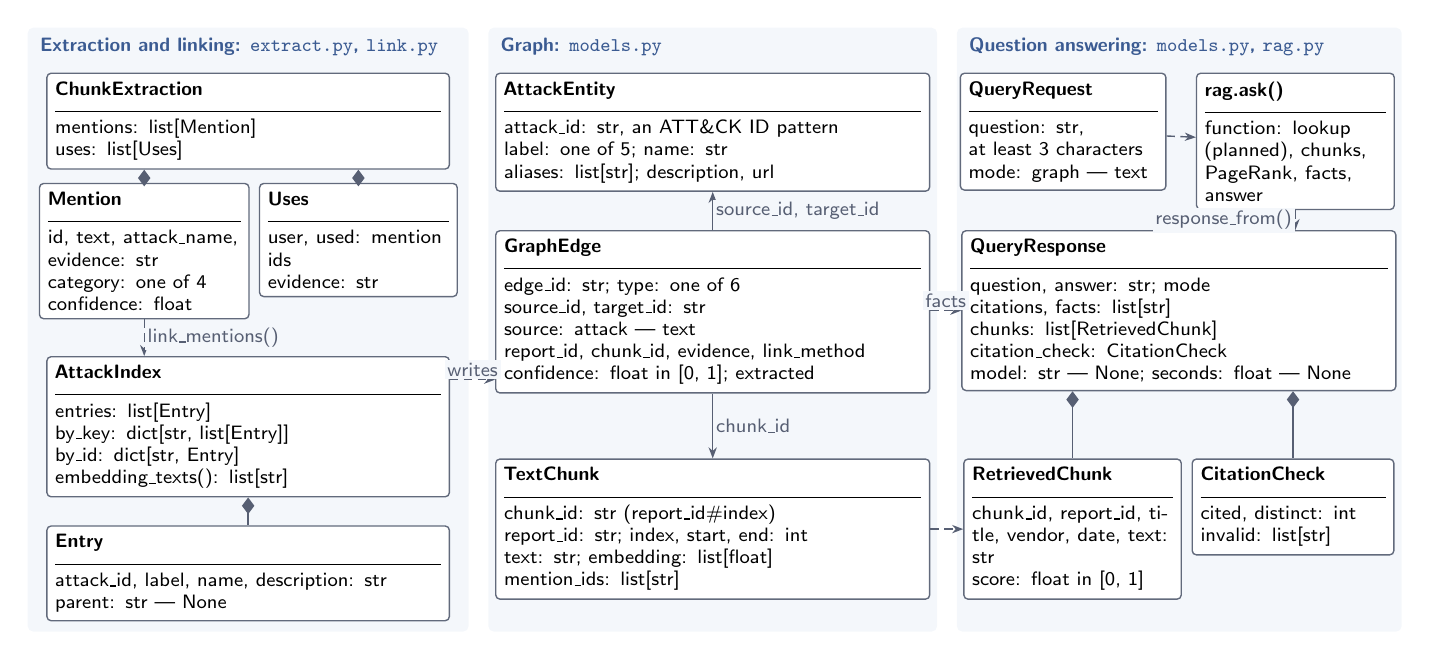
\begin{tikzpicture}[x=1cm, y=1cm]
\tikzset{cls/.style={draw=ink!70, fill=white, rounded corners=1.5pt, align=left, inner sep=3pt, font=\sffamily\scriptsize, line width=0.5pt, text width=#1, anchor=north},
  dep/.style={-{Stealth[length=4pt]}, dash pattern=on 3pt off 2pt, ink!75, line width=0.5pt},
  has/.style={{Diamond[length=6pt, width=4.5pt, fill=ink!75]}-, ink!75, line width=0.5pt},
  ref/.style={-{Stealth[length=4pt]}, ink!75, line width=0.5pt},
  lane/.style={font=\sffamily\scriptsize\bfseries, text=accent, anchor=north west, inner sep=0pt},
  elab/.style={font=\sffamily\scriptsize, fill=shade, inner sep=1pt}}
\begin{scope}[on background layer]
\path[fill=shade, rounded corners=2pt] (0,0.72) rectangle (5.6,-6.95);
\path[fill=shade, rounded corners=2pt] (5.85,0.72) rectangle (11.55,-6.95);
\path[fill=shade, rounded corners=2pt] (11.8,0.72) rectangle (17.45,-6.95);
\end{scope}
\node[lane] at (0.15,0.6) {Extraction and linking: \code{extract.py}, \code{link.py}};
\node[lane] at (6.0,0.6) {Graph: \code{models.py}};
\node[lane] at (11.95,0.6) {Question answering: \code{models.py}, \code{rag.py}};
\node[cls=4.9cm] (ce) at (2.8,0.15) {\cls{ChunkExtraction}{mentions: list[Mention]\\uses: list[Uses]}};
\node[cls=2.45cm] (me) at (1.48,-1.25) {\cls{Mention}{id, text, attack\_name, evidence: str\\category: one of 4\\confidence: float}};
\node[cls=2.3cm] (us) at (4.2,-1.25) {\cls{Uses}{user, used: mention ids\\evidence: str}};
\node[cls=4.9cm] (ai) at (2.8,-3.45) {\cls{AttackIndex}{entries: list[Entry]\\by\_key: dict[str, list[Entry]]\\by\_id: dict[str, Entry]\\embedding\_texts(): list[str]}};
\node[cls=4.9cm] (en) at (2.8,-5.6) {\cls{Entry}{attack\_id, label, name, description: str\\parent: str | None}};
\draw[has] (me.north |- ce.south) -- (me.north);
\draw[has] (us.north |- ce.south) -- (us.north);
\draw[dep] (me.south) -- node[elab, right]{link\_mentions()} (me.south |- ai.north);
\draw[has] (ai.south) -- (en.north);
\node[cls=5.3cm] (ae) at (8.7,0.15) {\cls{AttackEntity}{attack\_id: str, an ATT\&CK ID pattern\\label: one of 5; name: str\\aliases: list[str]; description, url}};
\node[cls=5.3cm] (ge) at (8.7,-1.85) {\cls{GraphEdge}{edge\_id: str; type: one of 6\\source\_id, target\_id: str\\source: attack | text\\report\_id, chunk\_id, evidence, link\_method\\confidence: float in [0, 1]; extracted}};
\node[cls=5.3cm] (tc) at (8.7,-4.75) {\cls{TextChunk}{chunk\_id: str (report\_id\#index)\\report\_id: str; index, start, end: int\\text: str; embedding: list[float]\\mention\_ids: list[str]}};
\draw[ref] (ge.north) -- node[elab, right]{source\_id, target\_id} (ae.south);
\draw[ref] (ge.south) -- node[elab, right]{chunk\_id} (tc.north);
\draw[dep] (ai.north east) ++(0,-0.3) coordinate (w) -- node[elab, above]{writes} (w -| ge.west);
\node[cls=2.4cm] (qr) at (13.15,0.15) {\cls{QueryRequest}{question: str,\\at least 3 characters\\mode: graph | text}};
\node[cls=2.3cm] (ask) at (16.1,0.15) {\cls{rag.ask()}{function: lookup (planned), chunks, PageRank, facts, answer}};
\node[cls=5.3cm] (qs) at (14.62,-1.85) {\cls{QueryResponse}{question, answer: str; mode\\citations, facts: list[str]\\chunks: list[RetrievedChunk]\\citation\_check: CitationCheck\\model: str | None; seconds: float | None}};
\node[cls=2.55cm] (rc) at (13.27,-4.75) {\cls{RetrievedChunk}{chunk\_id, report\_id, title, vendor, date, text: str\\score: float in [0, 1]}};
\node[cls=2.35cm] (cc) at (16.07,-4.75) {\cls{CitationCheck}{cited, distinct: int\\invalid: list[str]}};
\draw[dep] (qr) -- (ask);
\draw[dep] (ask.south) -- node[elab, left]{response\_from()} (ask.south |- qs.north);
\draw[has] (rc.north |- qs.south) -- (rc.north);
\draw[has] (cc.north |- qs.south) -- (cc.north);
\draw[dep] (ge.east |- qs.west) -- node[elab, above]{facts} (qs.west);
\draw[dep] (tc.east |- rc.west) -- (rc.west);
\end{tikzpicture}
\caption{Class diagram of the data models and the main classes. Diamond: contains. Solid arrow: refers to by key. Dashed arrow: uses or produces. The dashed arrows into the graph and question-answering models show how graph content maps onto them (a \code{GraphEdge} becomes a fact line of a \code{QueryResponse}; a \code{TextChunk} becomes a \code{RetrievedChunk}); in the built code those values travel as Neo4j rows, and the planned chat page fills the models.}\label{fig:classes}
\end{figure}

\section*{References}
{\footnotesize\begin{list}{}{\setlength{\leftmargin}{1.8em}\setlength{\labelwidth}{1.5em}\setlength{\labelsep}{0.3em}\setlength{\itemsep}{0pt}\setlength{\parsep}{0pt}\setlength{\topsep}{0pt}}
\item[{[1]}] L.\ Lange et al. AnnoCTR: A Dataset for Detecting and Linking Entities, Tactics, and Techniques in Cyber Threat Reports. LREC-COLING 2024, pp.\ 1147--1160.
\item[{[2]}] B.\ Jiménez Gutiérrez, Y.\ Shu, Y.\ Gu, M.\ Yasunaga, Y.\ Su. HippoRAG: Neurobiologically Inspired Long-Term Memory for Large Language Models. NeurIPS 37, 2024.
\item[{[3]}] T.\ H.\ Haveliwala. Topic-Sensitive PageRank. WWW 2002.
\item[{[4]}] H.\ Chen, S.\ F.\ Sultan, Y.\ Tian, M.\ Chen, S.\ Skiena. Fast and Accurate Network Embeddings via Very Sparse Random Projection. CIKM 2019.
\item[{[5]}] V.\ D.\ Blondel, J.-L.\ Guillaume, R.\ Lambiotte, E.\ Lefebvre. Fast Unfolding of Communities in Large Networks. J.\ Stat.\ Mech., 2008, P10008.
\item[{[6]}] Yu.\ A.\ Malkov, D.\ A.\ Yashunin. Efficient and Robust Approximate Nearest Neighbor Search Using Hierarchical Navigable Small World Graphs. IEEE TPAMI 42(4):824--836, 2020.
\item[{[7]}] S.\ Es, J.\ James, L.\ Espinosa Anke, S.\ Schockaert. RAGAs: Automated Evaluation of Retrieval Augmented Generation. EACL 2024 System Demonstrations, pp.\ 150--158.
\item[{[8]}] L.\ Zheng et al. Judging LLM-as-a-Judge with MT-Bench and Chatbot Arena. NeurIPS 2023 Datasets and Benchmarks.
\item[{[9]}] A.\ Panickssery, S.\ R.\ Bowman, S.\ Feng. LLM Evaluators Recognize and Favor Their Own Generations. NeurIPS 37, 2024.
\item[{[10]}] K.\ Wataoka, T.\ Takahashi, R.\ Ri. Self-Preference Bias in LLM-as-a-Judge. arXiv:2410.21819, 2024.
\item[{[11]}] B.\ Strom, A.\ Applebaum, D.\ Miller, K.\ Nickels, A.\ Pennington, C.\ Thomas. MITRE ATT\&CK: Design and Philosophy. MITRE, 2020.
\end{list}}
\end{document}
